\documentclass{article}
\usepackage[utf8]{inputenc}
\usepackage{natbib}
\usepackage{graphicx}
\usepackage{lastpage}
\usepackage{xcolor}
\usepackage{lipsum}
\usepackage[T1]{fontenc}
\usepackage{fancyhdr}
\usepackage{geometry}
\usepackage{url}
\usepackage[dutch]{babel}


\bibliographystyle{abbrv} %abbrvnat geeft problemen

\title{Software Project Management Plan}
\author{} %leave empty
\date{15 december 2014} %ok, manuele datum

\addtolength{\footskip}{1.3cm} % make more space for the footer
\pagestyle{fancyplain} % use fancy for all pages except chapter start
\lhead{}
\cfoot{
\includegraphics[height=1.3cm]{Small_Logo.png}} % right logo
\rfoot{\thepage}
\renewcommand{\headrulewidth}{0.3pt} % remove rule below header
\renewcommand{\footrulewidth}{0.3pt} % remove rule below header

\begin{document}

\makeatletter
\begin{titlepage}

\newcommand{\HRule}{\rule{\linewidth}{0.7mm}} % Defines a new command for the horizontal lines, change thickness here


\vspace*{1.2mm}

\center 

\includegraphics[scale=0.6]{Logo.png}\\[1cm] 
%---------------------------------------------------------------------------------------
%	HEADINGS SECTION
%----------------------------------------------------------------------------------------

\textsc{\LARGE Vrije Universiteit Brussel}\\[0.3cm] % Name of your university/college
\textsc{\large WE-DINF-6537}\\
\textsc{\large Project Software Engineering}\\
\textsc{\large Academiejaar 2014-2015}\\[0.3cm] 
%\textsc{\large Software Engineering}\\[0.7cm] % Major heading such as course name

%----------------------------------------------------------------------------------------
%	TITLE SECTION
%----------------------------------------------------------------------------------------

\HRule \\[0.4cm]
{ \huge \bfseries \@title \\[0.5cm] }
\HRule \\[0.5cm]
 
%----------------------------------------------------------------------------------------
%	AUTHOR SECTION
%----------------------------------------------------------------------------------------

\Large
% laat voorlopig nog even de namen/mailadressen op deze pagina staan
% eerst moeten we zien of er een beter alternatief is om de lege plek dan op te vullen
% anders laten we ze gewoon staan...

%volgens mij ziet het er zo heel goed uit, maar als ze echt wegmoeten mss vub logo groter maken? 
% => OK, ik vind het ook veter zo, we laten ze staan!
Douglas Horemans \textit{<dhoreman@vub.ac.be>}\\
Hannah Pinson \textit{<hpinson@vub.ac.be>}\\
Ivo Vervlimmeren \textit{<ivervlim@vub.ac.be>}\\
Noah Van Es \textit{<noahves@vub.ac.be>}\\
Pieter Steyaert \textit{<psteyaer@vub.ac.be>}\\

\vspace{0.6cm}


\includegraphics[scale=0.4]{VUB_schild.pdf}\\[0.5cm]

{\large 19 november 2014}
\vfill % Fill the rest of the page with whitespace

\end{titlepage}

\newpage
\section*{Versiegeschiedenis}
\addcontentsline{toc}{section}{Versiegeschiedenis}

\begin{center}
\begin{tabular}[t]{| c | c | c | c |}
    \hline
    \textbf{Versie} & \textbf{Datum} & \textbf{Auteurs\cite{note:author}} & \textbf{Beschrijving} \\
    \hline
    
    1.0     &  19/11/2014   &   \begin{tabular}{c} 
                                    Douglas Horemans \\
                                \end{tabular} & Eerste versie \\
    \hline
    2.0     &  15/12/2014   &   \begin{tabular}{c} 
                                    Douglas Horemans \\
                                \end{tabular} & tweede versie \\
    \hline
\end{tabular}
\end{center}
\newpage



\tableofcontents
\newpage


%%%%%%%%%%%%%%%%%%%%%%%%    FEED-BACK  %%%%%%%%%%%%%%%%%%%%%%%%%%%%%%
\newcommand{\comment}[1]{}


% --------> reeds aangepast

\comment{
%sectie 1.1
%- Citaties (ook verderop in document) komen na het laatste woord, voor de punt. In Latex:

   %      einde van de zin~\cite{xyz}.

%sectie 2.2
%- "Structuur van de Organisatie": het ene impliceert het andere

sectie 3.1
%- "die waar"
%- "Dit wordt verder besproken in? (zin niet afgewerkt)
%- erg veel tekst in verhalende vorm: het mag iets droger en meer 'to
%the point', het moet mogelijk zijn om snel informatie uit het document
%op te pikken

sectie 3.2
%- "...in een apart document, het Risk List (RL) document.": het is
%beter om dit aan te vullen in het huidige document.
%- De risk list mist projectgebonden risico?s. Tracht ervoor te zorgen dat de voorgestelde oplossingen meetbaar zijn.

sectie 3.3
%- De duurtijd van een vergadering is te groot. Een vergadering om na te gaan of een sprint al dan niet goed loopt, mag niet meer dan een half uur duren.

sectie 4.1
%- Is enkel de QAM verantwoordelijk voor het opsporen van inconsistenties en defecten?
- Hoe ga je als groep configuration management aanpakken?

%sectie 5
%- Is het niet mogelijk om de eerste sprint reeds te beschrijven? 

Algemeen:
Dit is een vrij uitgebreide eerste versie, met hier en daar nog (vaak zelf aangegeven) punten waar aanvulling noodzakelijk is. Eem werkplan ontbreekt. Probeer zo veel mogelijk aan te vullen voor volgende opleveringen. 
}



%%%%%%%%%%%%%%%%%%%%%%%%    NOTES TO SELF  %%%%%%%%%%%%%%%%%%%%%%%%%%%%%%

% nieuwe functie test manager toevoegen


%%%%%%%%%%%%%%%%%%%%%%%%%%%%%%%%%%%%%%%%%%%%%%%%%%%%% 1.INTRODUCTIE

\section{Introductie}

\subsection{Inleiding en Overzicht}
Het doel van dit softwareproject is het ontwikkelen van een webapplicatie die het enerzijds mogelijk maakt voor onderzoekers om wetenschappelijke publicaties te beheren en die anderzijds de netwerken van deze onderzoekers analyseert en op een aantrekkelijke manier visualiseert. Deze applicatie, die de naam SKRIBL draagt, wordt binnen het kader van het opleidingsonderdeel \emph{software engineering} gecre\"{e}erd gedurende het academiejaar 2014-2015. De rol van externe controle en klant worden hierbij vervuld door de titularis Ragnhild Van Der Straeten en de assistent Jens Nicolay van dit opleidingsonderdeel.\newline
\\
SKRIBL stelt gebruikers in staat om op een eenvoudige manier een lijst van eigen publicaties aan te leggen. Het is ook mogelijk publicaties van andere gebruikers en externe publicaties op te zoeken, te raadplegen en te bewaren. Bovendien kunnen alle publicaties geannoteerd worden, en kunnen ook niet-publicaties als slides en bijlagen aan de publicaties gerelateerd worden. Aan de hand van metadata analyseert SKRIBL de posities en onderlinge relaties binnen de wetenschappelijke wereld van de onderzoekers en hun publicaties. Dit laat SKRIBL enerzijds toe de meest relevante publicaties aan bepaalde gebruikers voor te stellen naargelang hun interesses en onderzoeksdomeinen aan de hand van een feedback-systeem dat hun voorkeuren leert kennen. Anderzijds zorgen deze analyses ervoor dat een gebruiker (zijn of haar eigen positie binnen) wetenschappelijke netwerken kan evalueren: aan de hand van de metadata kunnen interactieve grafen gecre\"{e}erd worden die het netwerk van de onderzoekers en de zwaartepunten binnen hun vakgebied weergeven, en gebruikers kunnen bovendien hun eigen statistieken raadplegen en visualiseren. De uiteindelijke applicatie zal zowel beschikbaar zijn via een standaard webinterface die eveneens geoptimaliseerd zal zijn voor mobiel gebruik. Daarnaast zal deze mobiele interface ook extra features ondersteunen die later in het ontwikkelingsproces zullen vastgelegd worden.\newline
\\
SKRIBL zal ontwikkeld worden door een team van vijf studenten in de computerwetenschappen volgens de principes van een Agile development software process. De totale werkperiode wordt opgedeeld in iteraties en sprints, waarbij het doel is een werkende parti\"{e}le versie van de software te ontwikkelen en daarbij telkens een zogeheten mijlpaal te bereiken. Het uiteindelijke doel van het totale project is het opleveren van een eindproduct dat aan alle vooropgestelde eisen van de klant voldoet en dat bovendien op ieder vlak van hoge kwaliteit is. Daarnaast zullen verschillende documenten betreffende het softwareproces opgemaakt en onderhouden worden en zal een deel van het werkproces publiek worden gemaakt via een website \citep{website:skribl} .Ten slotte zal er over de voortgang van het project ook telkens worden gecommuniceerd door middel van presentaties.


\subsection{Opleveringen}

De volgende documenten worden gedurende het project onderhouden en bij iedere iteratie opgeleverd:

\begin{itemize}
\item Software Project Management Plan (SPMP)
\item Software Test Plan (STD)
\item Software Requirements Specification (SRS)
\item Software Design Document (SDD)
\item Minutes van alle vergaderingen.
\end{itemize}

Aan het einde van iedere iteratie wordt ook telkens een werkende parti\"{e}le versie met de bijhorende broncode, documenten en unit-tests opgeleverd zoals bepaald in
\cite{Xtreport:organisatie}. Dit gebeurt via mail en valt onder de verantwoordelijkheid van de Project Manager. Daarnaast vindt er na iedere iteratie ook nog een presentatie plaats, waarvan de voorbereiding onder de verantwoordelijkheid van de Presentation Master valt. De data van opleveringen en presentaties zijn weergegeven in figuur \ref{Kalender}.

\begin{figure}[h!]
\centering
 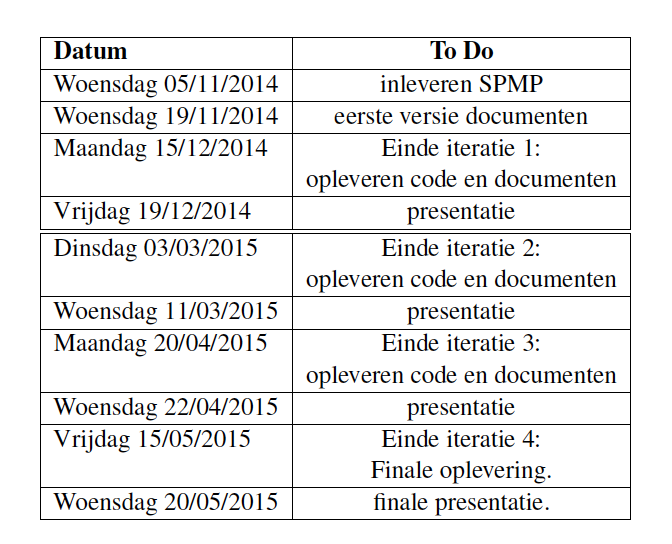
\includegraphics[width=120mm]{kalender.png}
 \caption{Vooropgestelde data van opleveringen en presentaties.}
 \label{Kalender}
\end{figure}

\subsection{Evolutie van het Software Project Management Plan}

Dit Software Project Management Plan is opgesteld volgens de IEEE 1085.1-1987 standaard,\citep{website:Cal-Poly}. In iedere iteratie zal het verder aangevuld worden, en voor iedere oplevering wordt een voorlopige  offici\"{e}le versie afgewerkt. In volgende versies zullen voornamelijk de onderdelen 4 (Technisch proces) en 5 (Werkpaketten en schema's) verder uitgewerkt worden. Suggesties voor toekomstige versies zijn geplaatst binnen vierkante haakjes en worden in cursief weergegeven.   

\clearpage

\subsection{Referentiemateriaal}
\begingroup
\renewcommand{\section}[2]{}% verwijdert titel sectie referenties
\bibliography{referenties}
\endgroup
 
\subsection{Definities en Afkortingen}
\begin{itemize}
\item SPMP: Software Project Management Plan 
\item STD:  Software Test Plan 
\item SRS: Software Requirements Specification 
\item SDD: Software Design Document 
\item RL: Risk List
\item PM: Project Manager
\item QA(M): Quality Assurance (Manager)
\item CM: Configuration Manager
\end{itemize}

 \clearpage

%%%%%%%%%%%%%%%%%%%%%%%%%%%%%%%%%%%%%%%%%%%%%%%%%%%%% 2.PROJECTORGANISATIE

\section{Projectorganisatie}
\subsection{Model van het softwareproces}

De applicatie zal gecre\"{e}erd worden door iteratieve ontwikkeling en incrementele oplevering, gestuurd door de principes van de agile development methode \cite{website:agile-process} . Concreet wordt het volledige proces opgedeeld in vier iteraties waarvoor de uiteindelijke doelen in grote lijnen vastliggen. Deze iteraties bevatten, afhankelijk van de totale duur, \'{e}\'{e}n of twee sprints. De sprints bestaan uit drie fasen die mogelijk deels overlappen: een plannings- en designfase, een uitvoeringsfase, en een test- en refactorfase. Een sprint beslaat een periode van twee tot vier weken. Het doel van iedere sprint is het ontwikkelen van een werkende parti\"{e}le versie en het bereiken van een zogenaamde mijlpaal:

\subsubsection*{Mijlpaal 1: inloggen en registreren mogelijk}

Nieuwe gebruikers kunnen een account aanmaken en geregistreerde gebruikers kunnen inloggen na invoer van correcte gebruikersnaam en wachtwoord.

\subsubsection*{Mijlpaal 2: eigen publicaties kunnen worden toegevoegd}
Gebruikers kunnen publicaties toevoegen zoals beschreven in scenario 1  \citep{Xtreport:organisatie}.
\subsubsection*{Mijlpaal 3: publicaties kunnen opgezocht, toegevoegd en geannoteerd worden}
Gebruikers kunnen publicaties van anderen opzoeken en bewaren zoals beschreven in scenario 3 \citep{Xtreport:organisatie}. Gebruikers kunnen publicaties annoteren en niet-publicaties (bijlagen, slides e.d.) kunnen worden gelinkt zoals beschreven in scenario 6 \citep{Xtreport:organisatie}.

\subsubsection*{Mijlpaal 4: metadata wordt gegenereerd en eenvoudig weergegeven}
Er worden automatisch up-to-date bibliometrische gegevens toegekend aan publicaties.
De relevantie van een publicatie voor een gebruiker kan gekwantificeerd worden en een top vijf kan op deze manier worden gegenereerd (statisch).
Voor iedere gebruiker worden statistische gegevens berekend en numeriek weergegeven.

\subsubsection*{Mijlpaal 5: netwerk wordt gecre\"{e}erd en gevisualiseerd}
Gebruikers en publicaties worden beschouwd als een netwerk, verbonden door standaard relaties als auteurschap, citaties, onderzoeksdomeinen ed. Aanpassingen aan dit netwerk worden consistent doorgevoerd.
Het netwerk van een gebruiker kan zo dan worden weergegeven als een interactieve graaf.

\subsubsection*{Mijlpaal 6: uitgebreide interactie en visualisatie mogelijk}
De relevantie-score van een publicatie wordt aangepast aan de voorkeuren van de gebruiker.
Gebruikers kunnen publicaties linken op manieren die de applicatie niet standaard voorziet.
De gebruiker kan grafieken laten genereren en exporteren.

\subsubsection*{Mijlpaal 7: mobiele interface en extra features}
Naast de standaard webinterface is er ook een interface voor mobiel gebruik. Bij deze interface wordt er rekening gehouden met de specifieke mogelijkheden en beperkingen van mobiele apparaten. In een later stadium van het project zal er worden beslist welke extra functionaliteit aan deze interface zal worden toegevoegd. \newline
\\

\begin{figure}[h!]
 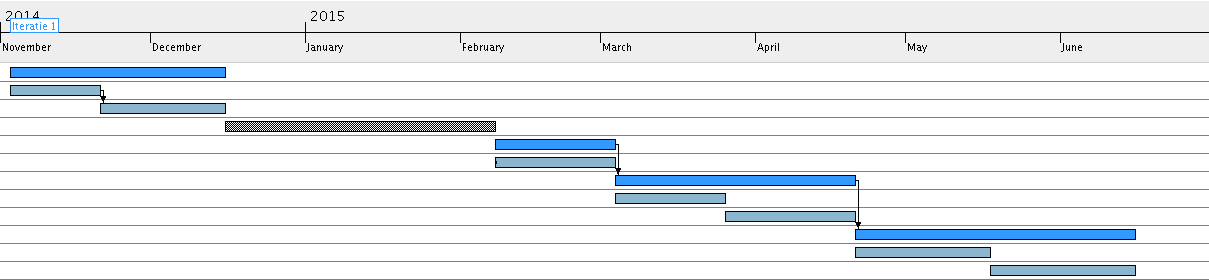
\includegraphics[width=150mm]{gantt_cropped.png}
 \caption{Gantt chart van het SKRIBL project. In blauw de geplande iteraties, in grijs de geplande sprints. \small{Afbeelding gegeneerd via Ganttproject, \emph{http://www.ganttproject.biz}}.}
 \label{GanttChart}
\end{figure}

\begin{table}[h!]
\begin{center}
\begin{tabular}{||c||c||c||c||c||c||}
	\hline
	\bf{Iteratie} & \bf{Sprint}  & \bf{Begin}  & \bf{Einde}  & \bf{Mijlpaal}   & \bf{Oplevering}  
	\\
	\hline
	\bf{1} & 1 & \bf{01/11/14} & 20/11/14 & 1: inloggen \& registeren & nee \\
	& 2 & 21/11/14 & \bf{15/12/14} & 2: eigen publicaties & \bf{ja}\\
	\hline
	\bf{2} & 3 & \bf{08/02/15} & \bf{03/04/15} & 3: publicaties  uitgebreid & \bf{ja} 	\\
	\hline
	\bf{3} & 4 & \bf{04/03/15} & 25/03/15 & 4: metadata & nee \\
	& 5 & 26/03/15 & \bf{20/04/15} & 5: netwerk & \bf{ja} \\
	\hline
	\bf{4} & 6 & \bf{21/04/15} & 17/05/15 & 6: interactie \& visualisatie & nee 	\\
	& 7 & 18/05/15 & \bf{15/06/15} & 7: mobiel & \bf{ja} 	\\
	\hline
\end{tabular}
 \end{center}
 \caption{Algemene planning van het ontwikkelingsproces.}
 \label{planning}
 \end{table}
 
De algemene planning van het project is te vinden in tabel \ref{planning} en deze planning is ook weergegeven in figuur \ref{GanttChart}. Bij deze planning worden de vooropgestelde scenario's niet chronologisch uitgewerkt. In plaats daarvan zijn scenario's of delen van scenario's gegroepeerd volgens te bereiken mijlpalen, en dit op zo'n manier dat alle scenario's aan het einde van het project ge\"{i}mplementeerd zullen zijn.
 

\subsection{Organisatie}

De verschillende leden van de groep nemen elk de twee (of een enkele keer drie) van de hieronder vermelde rollen op zich. Dit wil zeggen dat zij de eindverantwoordelijkheid dragen voor de vermelde aspecten van het ontwikkelingsproces. Daarnaast fungeert ieder lid ook voor twee of drie rollen als back-up persoon om opvolging en continu\"{i}teit binnen het project te verzekeren, en om de hoofdverantwoordelijken bij te staan. Ten slotte is ieder lid ook developer en schrijft hij/zij dus ook de unit testen voor de onderdelen die hij/zij zelf ontwikkelt. 

\subsubsection*{Project Manager}
\begin{itemize}
\item algemene co\"{o}rdinatie en planning
\item taakverdelingen
\item vastleggen, voorbereiden en leiden van vergaderingen
\item onderhouden van het SPMP
\item communicatie met end-user
\end{itemize}

\subsubsection*{Requirements Manager}
\begin{itemize}
\item analyseren van requirements: bijvoorbeeld informatie over journals en publicaties, documentformaten, enz. 
\item Het nauwkeurig oplijsten van requirements, op zo'n manier dat design en testing mogelijk is.
\item Het onderhouden van het SRS.
\end{itemize}

\subsubsection*{Configuration Manager}
\begin{itemize}
\item bepalen afspraken en conventies metasoftware en tools (e.g., github structuur, conventies voor code commenting) 
\item waken over consistentie en integratie van verschillende software onderdelen (in samenspraak met de software architect)
\end{itemize}

\subsubsection*{Software Architect}
\begin{itemize}
\item algemene architectuur van de software bepalen 
\item ontwerpen API's van de modules
\item onderhouden van het SDD
\end{itemize}


\subsubsection*{Quality Assurance Manager}
\begin{itemize}
\item algemene toezicht op kwaliteit van de code en de ontwikkelde software
\end{itemize}

\subsubsection*{Test Manager}
\begin{itemize}
\item verzamelen en inspecteren van de door de leden geschreven tests
\item onderhouden van STD
\end{itemize}

\subsubsection*{Database Manager}
\begin{itemize}
\item design en onderhoud database
\end{itemize}

\subsubsection*{Webmaster}
\begin{itemize}
\item (technisch) design en onderhoud van websites
\end{itemize}

\subsubsection*{Design en front-end}
\begin{itemize}
\item (creatief) design en ontwikkeling van GUI's en datavisualisaties
\end{itemize}

\subsubsection*{Document Master}
\begin{itemize}
\item overzicht en specificatie van documenten die opgeleverd moeten worden, in samenspraak met specifieke verantwoordelijke 
\item consistentie van de lay-out bewaken
\item minutes van vergaderingen opstellen 
\end{itemize}

\subsubsection*{Presentation Master}
\begin{itemize}
\item voorbereiding van structuren, slides en eventueel demo's voor de presentaties
\end{itemize}


\subsection{Grenzen en raakvlakken van de organisatie}

De titularis en assistent van het opleidingsonderdeel software engineering, Ragnhild Van Der Straeten en Jens Nicolay respectievelijk, vervullen samen enerzijds de rol van externe controle en anderzijds de rol van klant. \\

\noindent Om hen inzicht in het werkproces te geven onderhoudt de groep een website met een requirements dashboard en links naar de github repository en opgeleverde documenten. Deze website valt onder de verantwoordelijkheid van de webmaster.  \\

\noindent Aan het eind van elke iteratie worden de gevraagde bestanden en documenten opgeleverd en kort na iedere iteratie stelt de groep de voortgang en bereikte resultaten voor tijdens een presentatie. De communicatie en de oplevering valt onder de verantwoordelijkheid van de Project Manager. Het voorbereiden en in goede banen leiden van de presentaties is de taak van de Presentation Master. 

 \clearpage

\subsection{Projectverantwoordelijkheden}

\iffalse
dsaads
fdfdfds
\fi

\begin{table}[!h] 
  \begin{center}
    \begin{tabular}{| l || l | l |} 
      \hline
       {\bf Rol } &  {\bf Lead} &  {\bf  Back-up}  \\
      \hline
      Project Manager & Hannah & Pieter  \\
      \hline
      Configuration Manager & Pieter &  Douglas \\
      \hline
      Requirements Manager & Hannah & Noah \\
      \hline
      Software Architect & Noah & Ivo  \\
      \hline
      Quality Assurance Manager & Noah &  Pieter \\
      \hline
      Test Manager & Douglas &  Ivo \\
      \hline
       Database Manager & Ivo & Hannah  \\
      \hline
       Webmaster & Douglas & Hannah \\
      \hline
     Design en front-end & Pieter & Douglas \\
      \hline
       Document master & Ivo & Noah   \\
      \hline
        Presentation master & Douglas & Noah \\
      \hline
    \end{tabular}
  \end{center}
  \caption{Verantwoordelijkheden binnen het project: lead en back-up rollen.}
  \label{rolverdeling}
 \end{table}







%%%%%%%%%%%%%%%%%%%%%%%%%%%%%%%%%%%%%%%%%%%%%%%%%%%%% 3.MANAGEMENTPROCES

\section{Managementproces}

%%%

\subsection{Beperkingen, objectieven en prioriteiten}

\noindent De baseline van het management proces is als volgt samen te vatten: eerst en vooral staat het verwezenlijken van prioritaire doelen en bijhorende hoge kwaliteit voorop; het streven naar resultaten met een lage prioriteit gebeurt na samenspraak met de groep en enkel als ieder lid de taak voor zichzelf haalbaar vindt. De project manager verbindt zich ertoe dit voor ieder lid afzonderlijk op te volgen. De Quality Assurance Manager waakt verder over de kwaliteit van de behaalde doelen. 



%%%
\subsection{Risicomanagement}
\label{subsec:risico}
Risico's zullen op volgende manieren gedetecteerd en opgelijst worden:

\begin{itemize}
\item door het nagaan van de risico's voor andere, gelijkaardige softwareprojecten
\item door iedere openingsvergadering enkele minuten aan het onderwerp te besteden 
\item door het aandragen van verwachte risico's door leden aan de PM 
\end{itemize}

De risico's zullen opgevolgd worden door de PM. \newline


\subsubsection{algemene risico's}

\subsubsection*{Een te grote werklast}
\begin{itemize}
\item waarschijnlijkheid: groot
\item melding: Groepsleden geven aan wanneer de werklast voor hen te groot dreigt te worden.
\item oplossing: Aan het begin van iedere sprint worden de opdrachten geprioriteerd. Indien de werkdruk te hoog zou worden kunnen minder belangrijke opdrachten weggelaten of opgeschoven worden. De laatste sprint laat ruimte voor het uitvoeren van eventueel onafgewerkte features. Tijdens blok- en examenperiodes en tijdens vakanties wordt er niet verwacht van de groepsleden aan het project te werken.
\end{itemize}

\subsubsection*{Onvoldoende ervaring of kennis}
\begin{itemize}
\item waarschijnlijkheid: groot
\item melding: Groepsleden geven duidelijk aan wanneer zij het gevoel hebben dat het hen aan de nodige kennis of ervaring ontbreekt. De Project Manager maakt ruimte in de planning voor het wegwerken van de achterstand (indien mogelijk) en geeft dit ook expliciet als taak op.
\item oplossing: Het herhalen van cursussen en/of het volgen van online tutorials.
\end{itemize}

\subsubsection*{Afwezigheid of ziekte}
\begin{itemize}
\item waarschijnlijkheid: groot
\item melding: Groepsleden laten zo vroeg mogelijk weten wanneer en hoelang zij afwezig zullen zijn.
\item oplossing: Voor iedere rol is er een persoon aangeduid als back-up. Deze volgt de activiteiten van de hoofdverantwoordelijke op en kan deze rol overnemen indien nodig.
\end{itemize}

\subsubsection*{Eindresulaat is niet gebruiksvriendelijk}
\begin{itemize}
\item waarschijnlijkheid: gemiddeld
\item melding: De beta versies zullen worden voorgelegd aan enkele externe testers, zoals bereidwillige assistenten, maar ook personen die niet geaffilieerd zijn aan de wetenschappelijk wereld.
\item oplossing: De feedback van deze testers wordt gebruikt om aanpassingen aan het product door te voeren
\end{itemize}

\subsubsection{projectgebonden risico's}

\subsubsection*{vorm (meta)data niet voldoende consistent}
\begin{itemize}
\item waarschijnlijkheid: groot
\item beschrijving: de door gebruikers ingevoerde data is niet van een consistente vorm, e.g. de ene gebruiker geeft als universiteit 'VUB', de andere 'Vrije Universiteit Brussel'; de ene geeft auteurs met initialen, de andere met voornamen voluit etc. Dit bemoeilijkt het vinden van relaties om het netwerk van een gebruiker op te bouwen.
\item oplossing: Waar mogelijk het verwachte formaat specificeren of de keuzemogelijkheden beperken; eventueel reeds in het systeem aanwezige data als optie voorstellen.
\end{itemize}




%%%
\subsection{Opvolging, controle en communicatie}

Per sprint worden standaard twee vergadermomenten voorzien waarbij het hele team aanwezig is: een openingsvergadering en een follow-up vergadering. Dit komt neer op drie tot vier sprintbijeenkomsten per maand. De openingsvergadering vindt plaats aan het begin van de sprintperiode. De follow-up vergadering vindt plaats tussen midden en eind van de sprintperiode, d.w.z. aan het eind van de uitvoeringsfase en in het begin van de refactor- en testfase.\\
\\
\noindent De openingsvergadering bestaat uit de volgende componenten: \\
- deel 1 (ong. 45 min.):
\begin{itemize}
\item opening en overlopen agendapunten
\item micropresentaties (belichten de aspecten van het ontwikkelingsproces waarvoor het betreffende groepslid verantwoordelijk is)
\item variabele agendapunten en opmerkingen, zoals op te leveren documenten, afspraken e.d.
\end{itemize}
\noindent  -deel 2 (ong. 45 min):
\begin{itemize}
\item design en planning van de sprint
\item taakverdelingen
\item overlopen van risico's
\end{itemize}

\noindent De follow-up vergadering bestaat uit volgende componenten:\\
- (ong. 30 min.):
\begin{itemize}
\item opening en overlopen agendapunten
\item micropresentaties en reeds uitgevoerde taken
\item aanpak van quality assurance en testing 
\item overlopen van plan voor configuratie, integratie en eventueel oplevering
\item verwachte problemen 
\item eventuele (her)verdeling van taken en nieuwe acties 
\end{itemize}

\noindent  Naast de sprintbijeenkomsten kunnen er bijeenkomsten plaatsvinden tussen de groepsleden onderling, om deelaspecten van het project te bespreken of om bijvoorbeeld presentaties voor te bereiden. Daarnaast kan de QA Manager ook een korte reviewsessie organiseren met de eindverantwoordelijke van een bepaald onderdeel mocht de kwaliteit ervan betwist worden. \\

Doorlopende en overzichtelijke communicatie wordt verzekerd door het gebruik van enkele hiervoor ontwikkelde tools en communicatieplatformen. De (huidige) selectie van communicatiemiddelen werd na overleg binnen het volledige team gekozen uit een lijst met voorstellen samengesteld door de configuration manager. De keuzes werden ge\"{i}nspireerd door de eerdere ervaring van teamleden binnen kleinere softwareprojecten en startups. 

\subsubsection*{Algemene communicatie \& persoonlijke communicatie : Slack}
\begin{figure}[h!]
\centering
 
\includegraphics[width=50mm]{slack.png}
\end{figure}

\noindent Slack is een zeer eigentijds communicatieplatform, veelal gebruikt door nieuwe startups. Mededelingen over verschillende onderwerpen worden gegroepeerd in zogenoemde kanalen. Bovendien biedt Slack een waaier van integraties aan voor andere development- en communicatiediensten. Skribl gebruikt op dit moment 7 kanalen met individuele integraties naar Blossom, Github, Trello, Google Docs en Google Hangouts.\\
\noindent  Als alternatieven werden mail, Facebook, Google Groups, IRC, Skype en BaseCamp onderzocht. Geen van deze platformen biedt een degelijke uitgebreide integratie met third-parties aan, hetgeen de doorslag gaf voor Slack.

\clearpage

\subsubsection*{Algemeen takenbeheer : Trello}

\begin{figure}[h!]
\centering
 
\includegraphics[width=50mm]{trello_logo.png}
\end{figure}

\noindent Deze applicatie stelt een gebruiker en/of team in staat om lijstjes aan te maken met entries die gemakkelijk van lijstje kunnen verplaatst worden. Elke entry kan gekoppeld worden aan een of meerdere teamgenoten, kan een label krijgen, een deadline, etc. Deze tool wordt gebruikt voor alle task management die niet rechtstreeks met de development van de applicatie te maken heeft. 
\noindent Als alternatief werd Kanbanize besproken, maar vanwege de sterke integratie met Slack werd toch voor Trello geopteerd.


\subsubsection*{Opvolging agile development: Blossom}

\begin{figure}[h!]
\centering
 
\includegraphics[width=50mm]{blossom.png}
\end{figure}

\noindent  Blossom is een project management tool, specifiek ontwikkeld voor agile software processen. Met deze applicatie is het mogelijk lijsten met te ontwikkelen features op te stellen, aan deze features ontwikkelaars en deadlines toe te wijzen, en vervolgens de status van het ontwikkelingsproces aan te passen en op te volgen. Bovendien geeft Blossom ook per feature performantiestatistieken (cycle time performance analytics) weer. \\
\\
Blossom is een betalende applicatie. Na overleg met een van de founders van Blossom werd echter aan de leden van SKRIBL  voor academische doeleinden het gratis gebruik ervan toegestaan tot het einde van het academiejaar.  \\
Het team vond het zinvol om buiten Trello een gerichte tool te gebruiken voor het agile development proces. Voor Blossom is er een integratie aanwezig met GitHub en Slack, waardoor deze management tool de voorkeur van het team wegdroeg. 

\clearpage

\subsubsection*{Beheren van documenten: Google Drive \& Share\LaTeX}

\begin{figure}[h!]
\centering
 
\includegraphics[width=50mm]{google_drive.jpg}
\end{figure}

\noindent Door gemeenschappelijk in de cloud te werken met alle services van Google Drive (Docs, Spreadsheets of Presentaties) kunnen documenten collectief en in real-time aangepast en beheerd worden. Op deze manier wordt duplicatie vermeden en heeft iedereen steevast de laatste versie van een werkdocument. Documenten waarvan de inhoud afgewerkt is, worden door de document master(s) voor oplevering van een consistente en academische lay-out voorzien door gebruik van Share\LaTeX.\\
Als alternatief werd Evernote beschouwd, maar deze biedt niet dezelfde collectieve en real-time features als Google Drive. 
 
 
 \subsubsection*{Automatische code review: CodeClimate}

\begin{figure}[h!]
\centering
 
\includegraphics[width=50mm]{codeClimate.jpg}
\end{figure}

\noindent CodeClimate is een tool die, eens gekoppeld aan github, automatisch javascript code inspecteert en vervolgens rapporten genereert over de stijl en kwaliteit van deze code. CodeClimate biedt op die manier een objectieve analyse van de geschreven broncode. De teamleden kunnen de feedback van CodeClimate gebruiken om de kwaliteit van hun code te verbeteren, nog voor de Quality Assurance Manager deze hoeft te inspecteren.  

 
  \clearpage
 
 
%%%%%%%%%%%%%%%%%%%%%%%%%%%%%%%%%%%%%%%%%%%%%%%%%%%%% TECHNISCH PROCES

\section{Technisch proces}

\subsection{Technische tools en technieken}

Voor de ontwikkeling van SKRIBL wordt enkel gebruik gemaakt van JavaScript, HTML5 en CSS, en de daarbij horende open-sources frameworks en bibliotheken die nodig worden geacht. GitHub, ge\"{i}ntegreerd met Slack en Blossom, fungeert als repository en gedeeltelijk als collaboration tool. Onder leiding van de configuration manager wordt het ingezet als platform voor version-control, issue tracking en reviewing. Merging-issues en bugs worden volgens de standaard methoden van het platform behandeld. \\
\\
De conventies voor documentatie en code commenting worden opgesteld door de configuration manager (CM) en de quality assurance manager (QAM). Hierbij wordt gebruikt gemaakt van JSDocs. \\
\\
De test manager (TM) verzamelt de unit testen geschreven door de afzonderlijke teamleden, en houdt het overzicht over het gehele testproces. Hierbij wordt gebruik gemaakt van het jasmine testing framework. Meer informatie hieromtrent is te vinden in het STD.
\\
De quality assurance manager zal verder defecten en inconsistenties opsporen om de kwaliteit van de ontwikkelde onderdelen te garanderen. Dit zal gebeuren door:
\begin{itemize}
\item de kwaliteit van de geschreven op te volgen aan de hand van CodeClimate
\item na te gaan of alle modules correct worden ge\"{i}mplementeerd zoals omschreven in het SDD
\item te controleren dat aan alle vooropgestelde requirements voldaan is (zoals opgelijst in het SRS)
\end{itemize}
Automatische code-inspectie wordt uitgevoerd door de CodeClimate tool. Een door CodeClimate gerapporteerde  A of B wordt door het team als voldoende beschouwd. Indien de code van lagere kwaliteit is (of wanneer de QAM andere significante problemen vaststelt) wordt de code bijgeschaafd door het desbetreffende teamlid, eventueel volgens de richtlijnen van de QAM.
\\
Meer informatie over de syseemomgeving, de gebruikte database e.d. is te vinden in het SDD.



 \clearpage
%%%%%%%%%%%%%%%%%%%%%%%%%%%%%%%%%%%%%%%%%%%%%%%%%%%%% WERKPAKETTEN EN SCHEMA'S
\section{Werkpaketten en schema's }

\noindent [{\it Dit onderdeel zal na de opening van iedere sprint verder aangevuld worden.}] \newline
\\
\noindent De werkpakketten en planningen voor iedere sprint zullen weergegeven worden in eenvoudige Gantt charts. De lengte van de balkjes op het diagram stemt hierbij overeen met de verwachte werklast voor elke opdracht. 1 eenheid op het diagram komt overeen met 1 dag, waarbij 1 dag beschouwd als de gemiddelde werkdag van een student. Aangenomen wordt dat er op deze dag ruwweg twee uur aan de opdracht kan gespendeerd worden. De verwachte werklast wordt bepaald op de openingsvergadering van de sprint door een eenvoudig systeem van stemming en gemiddeldes. \newline

%
\subsection{Sprint 1:  Inloggen en Registreren}

Figuur \ref{gantt_S1} geeft de planning voor de eerste sprint weer. Deze sprint loopt van 1 november 2014 (notatie 11/01/14)  tot 20 november 2014 (notatie 11/20/14). Deze sprint heeft als mijlpaal 'mijlpaal 1: inloggen en registreren' en implementeert volgende features:
\begin{itemize}
\item registratie
\item login/logout
\item accountbeheer
\item taal
\end{itemize}

\noindent De bijhorende requirements zijn te vinden in het Software Requirements Specification (SRS) document. \newline
\\
\noindent Zoals op figuur \ref{gantt_S1}  is af te lezen, is er op datum 11/18/14 en grote achterstand in het ontwikkelingsproces. Deze achterstand heeft vier oorzaken: 
\begin{itemize}
\item het uitzoeken en installeren van de benodigde bibliotheken en software duurde langer dan verwacht
\item een van de teamleden was enkele dagen ziek
\item het ontbrak enkele teamleden aan de juiste kennis, onder meer in het gebruik van JavaScript, waardoor er extra tijd nodig was om deze zaken bij te spijkeren 
\item taken die niet in deze planning zijn opgenomen, onder meer het schrijven van de op te leveren documenten, bleken zeer tijdrovend te zijn
\end{itemize}
De PM zal deze situatie opvolgen en trachten te remedi\"{e}ren. In samenspraak met het team zullen enkele minder prioritaire requirements uitgesteld worden. 


\begin{figure}[h!]
\centering
 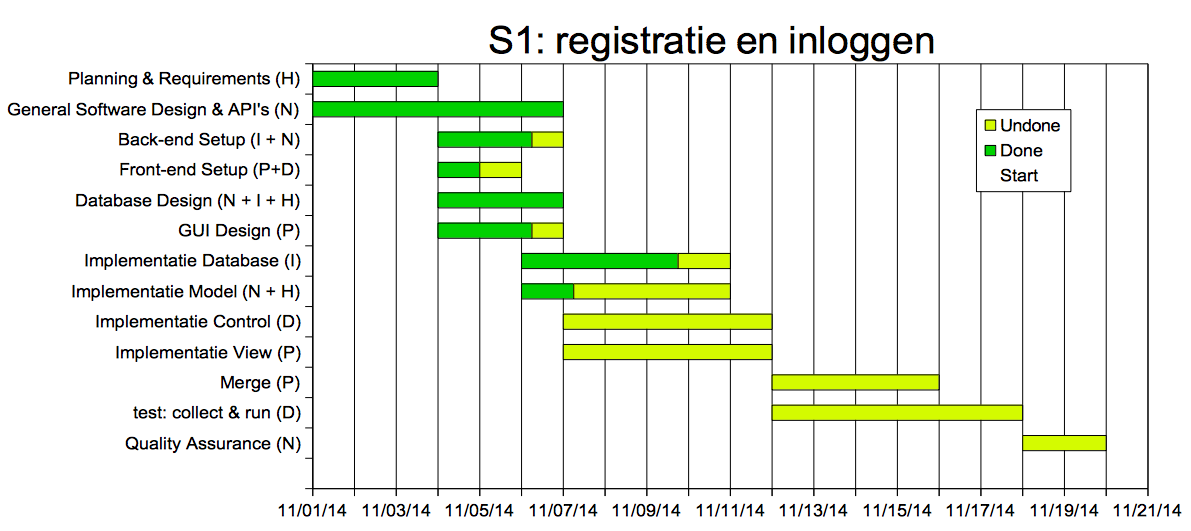
\includegraphics[scale=0.4]{Gantt_S1_19nov.png}
 \caption{Gantt chart voor sprint 1, op datum 11/18/14 (18 november 2014), einde van de sprint. Links van het diagram een korte beschrijving van de taak en de eerste letter van de voornaam van het corresponderende teamlid. Figuur gecre\"{e}erd met OpenOffice Calc.}
 \label{gantt_S1}
\end{figure}


\subsection{Sprint 2:  Publicatie uploaden}

Figuur \ref{gantt_S2_20nov} geeft de planning voor de tweede sprint weer, inclusief remedi\"{e}ring voor de achterstand opgelopen tijdens sprint 1. Sprint 2 loopt van 20 november 2014 (notatie 11/20/14)  tot 15 december 2014 (notatie 12/15/14). Deze sprint heeft als mijlpaal 'mijlpaal 2: publicatie toevoegen' en implementeert volgende features:
\begin{itemize}
\item toevoegen van publicatie in PDF of Bibtex formaat + metadata extractie en manuele aanvulling
\end{itemize}

\noindent De bijhorende requirements zijn te vinden in het Software Requirements Specification (SRS) document. 

\begin{figure}[h!]
\centering
 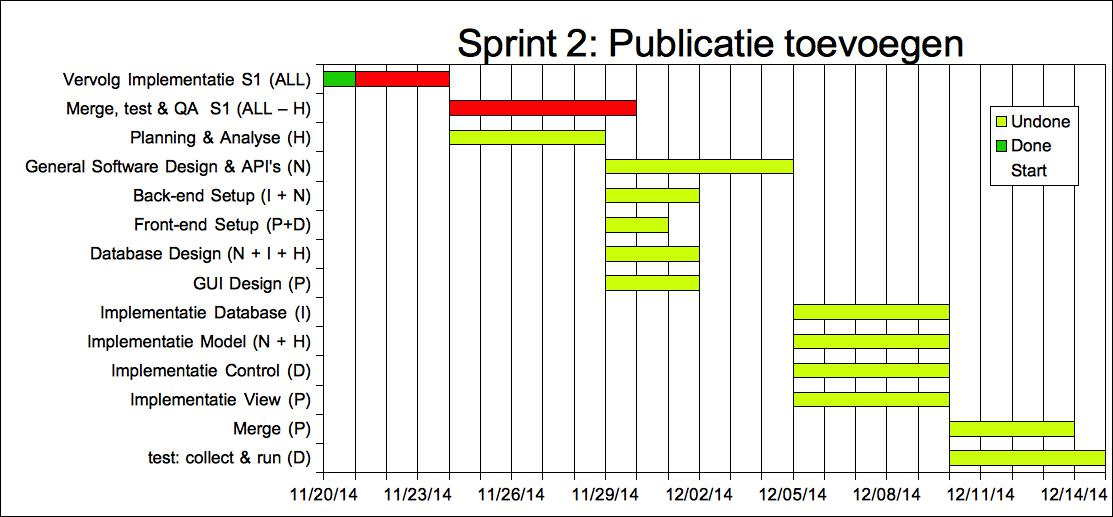
\includegraphics[scale=0.4]{Gantt_S2_20nov.jpg}
 \caption{Gantt chart voor sprint 2, op datum 20 november 2014, begin van de sprint. De rode balkjes corresponderen met de weg te werken achterstand in sprint 1. Figuur gecre\"{e}erd met OpenOffice Calc.}
 \label{gantt_S2_20nov}
\end{figure}

\noindent Aan het einde van de sprint 2, datum 20 november, is niet aan alle hoog en gemiddeld geprioriteerde requirements voor sprint 2 voldaan. Zoals te zien in figuur \ref{gantt_S2_15dec} is sprint 1 echter volledige afgerond en is de daarbij opgelopen achterstand grotendeels weggewerkt. 

\begin{figure}[h!]
\centering
 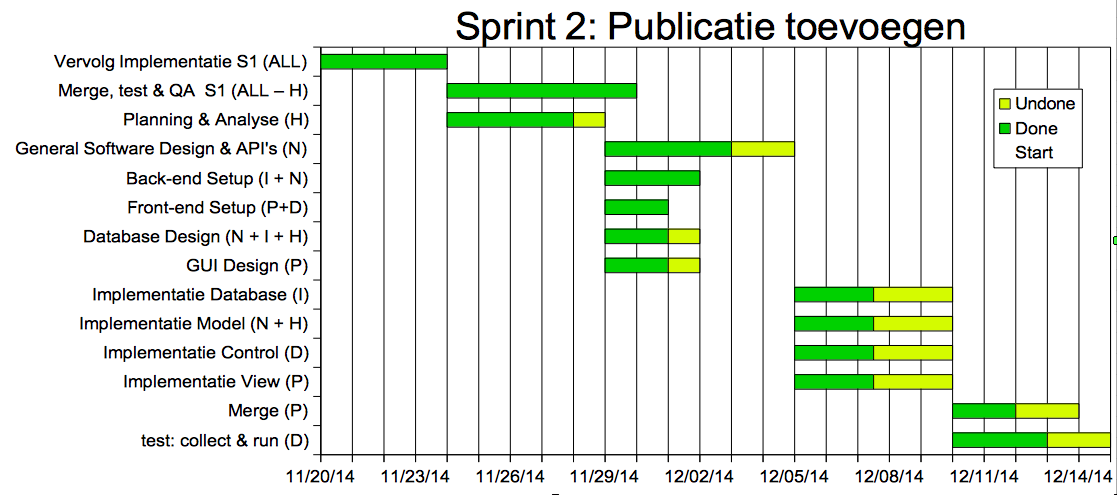
\includegraphics[scale=0.4]{Gantt_S2_15dec.png}
 \caption{Gantt chart voor sprint 2, op datum 15 december 2014, einde van de sprint. Figuur gecre\"{e}erd met OpenOffice Calc.}
 \label{gantt_S2_15dec}
\end{figure}

\clearpage
\subsection{Sprint 3:  Bibliotheek}

Figuur \ref{gantt_S3_2maart} geeft de planning voor de implementatie van de derde sprint weer, inclusief remedi\"{e}ring voor de achterstand opgelopen tijdens sprint 2. Sprint 3 loopt van 9 februari 2015  tot 2 maart 2015, en heeft als mijlpaal 'mijlpaal 3: bibliotheek' (zie SRS). De werkpaketten, deels gebaseerd op deze Gantt chart, zijn weergegeven in \ref{tabelS3}. Figuur \ref{pie_S3} ten slotte geeft een samenvatting van de re\"{e}le werkuren voor sprint 3. De geplande werklast was (met opzet) te hoog; dit blijkt ook uit het feit dat de doelstellingen voor deze sprint slechts gedeeltelijk behaald zijn. Volgende planningen zullen opgesteld worden met als richtgetal 30u per persoon per sprint, of ongeveer 10u per persoon per week. 

\begin{figure}[h!]
\centering
 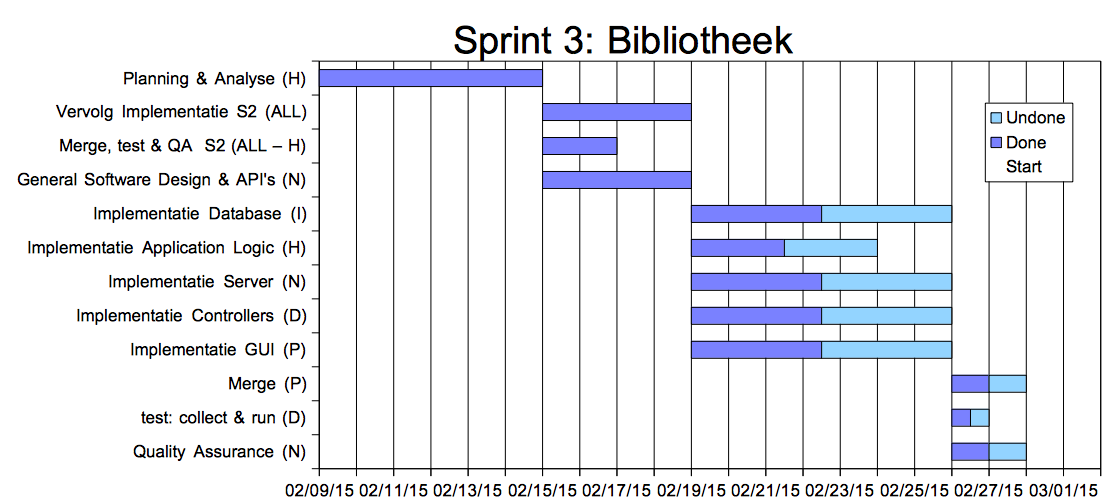
\includegraphics[scale=0.4]{Gantt_S3_2maart.png}
 \caption{Gantt chart voor sprint 3, op datum 02 maart 2015, einde van de sprint. Figuur gecre\"{e}erd met OpenOffice Calc.}
 \label{gantt_S3_2maart}
\end{figure}


\begin{table}[!h] 
  \begin{center}
    \begin{tabular}{|p{4cm}|p{3cm}|p{3cm}|p{3cm}|} 
      \hline
       {\bf Type } &  {\bf Berekening duur} &  {\bf  Geplande duur} &   {\bf Re\"{e}le duur aan einde sprint} \\
           \hline
      Taken algemeen: planning, documenten, etc.& planning en analyse (10u)  + 4u per doc + 1u pp overig & 10+16+5 = 31u & $\pm 33$u  \\
         \hline
         Bijscholing \& tutorials & 2u pp & 10u & $\pm 5$ u \\
           \hline
         Vergadering & 2 maal 1u pp & 10u & $\pm 8$ u \\
         \hline
         Implementatie, zie fig. \ref{gantt_S3_2maart} & 2u per eenheid * aantal toegewezen teamleden & 133u & $\pm 100$u (implementatie onvolledig) \\
   \hline
       Totaal & &  $\pm 185$u,  37u pp & $\pm 150$u, 30u pp (via Toggl) \\
   \hline
    \end{tabular}
  \end{center}
  \caption{Geplande en re\"{e}le werkpaketten sprint 3.}
  \label{tabelS3}
 \end{table}


\begin{figure}[h!]
\centering
 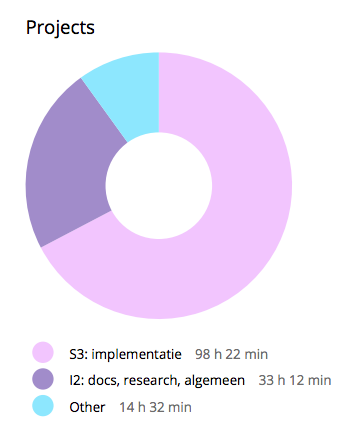
\includegraphics[scale=0.6]{Toggl_Pie_S3.png}
 \caption{Pie chart met re\"{e}le werkpaketten voor sprint 3, op datum 02 maart 2015, einde van de sprint. Figuur gecre\"{e}erd via Toggl. }
 \label{pie_S3}
\end{figure}


\end{document}
